\documentclass[]{standalone}
\usepackage{amsmath}
\usepackage{graphicx}
\usepackage[pdf]{pstricks}
\usepackage{pgfplots}
\pgfplotsset{compat=newest}
\usepgfplotslibrary{fillbetween}
%% the following commands are needed for some matlab2tikz features
\usetikzlibrary{plotmarks}
\usetikzlibrary{arrows.meta}
\usepgfplotslibrary{patchplots}
\usetikzlibrary{decorations.text}
\usetikzlibrary{shapes.multipart}

\newcommand{\logLogSlopeTriangle}[5]
{
	% #1. Relative offset in x direction.
	% #2. Width in x direction, so xA-xB.
	% #3. Relative offset in y direction.
	% #4. Slope d(y)/d(log10(x)).
	% #5. Plot options.
	
	\pgfplotsextra
	{
		\pgfkeysgetvalue{/pgfplots/xmin}{\xmin}
		\pgfkeysgetvalue{/pgfplots/xmax}{\xmax}
		\pgfkeysgetvalue{/pgfplots/ymin}{\ymin}
		\pgfkeysgetvalue{/pgfplots/ymax}{\ymax}
		
		% Calculate auxilliary quantities, in relative sense.
		\pgfmathsetmacro{\xArel}{#1}
		\pgfmathsetmacro{\yArel}{#3}
		\pgfmathsetmacro{\xBrel}{#1-#2}
		\pgfmathsetmacro{\yBrel}{\yArel}
		\pgfmathsetmacro{\xCrel}{\xArel}
		%\pgfmathsetmacro{\yCrel}{ln(\yC/exp(\ymin))/ln(exp(\ymax)/exp(\ymin))} % REPLACE THIS EXPRESSION WITH AN EXPRESSION INDEPENDENT OF \yC TO PREVENT THE 'DIMENSION TOO LARGE' ERROR.
		
		\pgfmathsetmacro{\lnxB}{\xmin*(1-(#1-#2))+\xmax*(#1-#2)} % in [xmin,xmax].
		\pgfmathsetmacro{\lnxA}{\xmin*(1-#1)+\xmax*#1} % in [xmin,xmax].
		\pgfmathsetmacro{\lnyA}{\ymin*(1-#3)+\ymax*#3} % in [ymin,ymax].
		\pgfmathsetmacro{\lnyC}{\lnyA+#4*(\lnxA-\lnxB)}
		\pgfmathsetmacro{\yCrel}{\lnyC-\ymin)/(\ymax-\ymin)} % THE IMPROVED EXPRESSION WITHOUT 'DIMENSION TOO LARGE' ERROR.
		
		% Define coordinates for \draw. MIND THE 'rel axis cs' as opposed to the 'axis cs'.
		\coordinate (A) at (rel axis cs:\xArel,\yArel);
		\coordinate (B) at (rel axis cs:\xBrel,\yBrel);
		\coordinate (C) at (rel axis cs:\xCrel,\yCrel);
		
		% Draw slope triangle.
		\draw[#5]   (A)-- node[pos=0.5,anchor=north] {1}
		(B)-- 
		(C)-- node[pos=0.5,anchor=west] {#4}
		cycle;
	}
}

\begin{document}
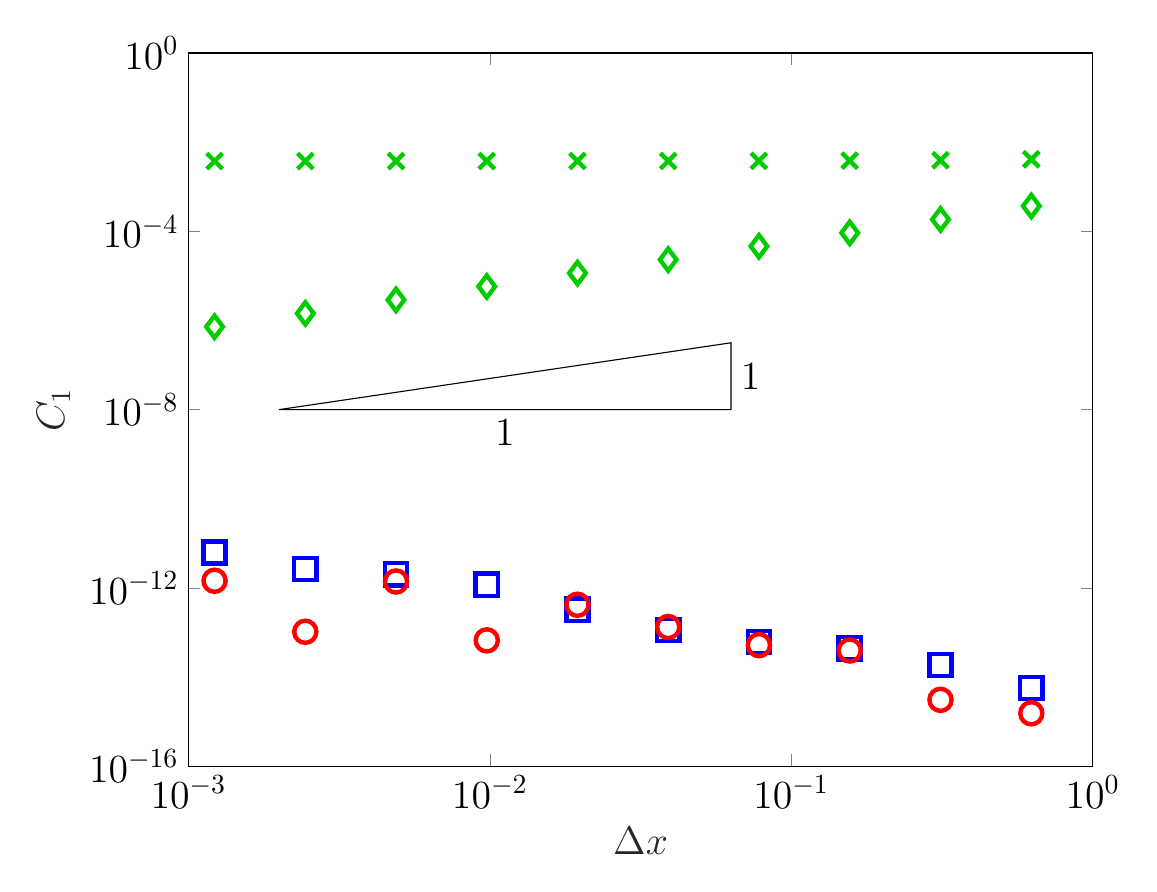
\begin{tikzpicture}
\tikzstyle{every node}=[font=\Large]
\begin{axis}[%
width=4.521in,
height=3.566in,
at={(0.758in,0.481in)},
every axis plot/.append style={ultra thick},
scale only axis,
xmode=log,
xmin=0.001,
xmax=1,
xtick={0.0001,  0.001,   0.01,    0.1,      1,     10},
xminorticks=false,
xlabel style={font=\color{white!15!black}},
xlabel={\Large $\Delta x$},
ymode=log,
ymin=1e-16,
ymax=1,
ytick={ 1e-16,  1e-12,  1e-08, 0.0001,      1},
yminorticks=true,
ylabel style={font=\color{white!15!black}},
ylabel={\Large $C_1$},
axis background/.style={fill=white},
legend style={at={(0.03,0.97)}, anchor=north west, legend cell align=left, align=left, draw=white!15!black}
]

\logLogSlopeTriangle{0.6}{0.5}{0.5}{1}{black};

\addplot [color=blue, draw=none, mark=square, mark size=4pt, mark options={solid, blue}]
  table[row sep=crcr]{%
5.05050505050505	3.56733880835235e-11\\
2.51256281407035	5.12803429349633e-15\\
1.2531328320802	5.29212229594127e-15\\
0.625782227784731	5.75293294483955e-15\\
0.312695434646654	1.84815007742139e-14\\
0.156298843388559	4.43997786684761e-14\\
0.0781372089388967	6.06235062150581e-14\\
0.0390655519962497	1.13374814721569e-13\\
0.0195320129692566	3.24676925344885e-13\\
0.00976581573858864	1.18307791711648e-12\\
0.00488286018418149	2.02072591105225e-12\\
0.00244141817098716	2.68072254395498e-12\\
0.00122070610523951	6.25791459992604e-12\\
};


\addplot [color=red, draw=none, mark=o, mark size=4pt, mark options={solid, red}]
  table[row sep=crcr]{%
5.05050505050505	2.29966242602921e-10\\
2.51256281407035	1.09744947528462e-15\\
1.2531328320802	2.42045514925841e-15\\
0.625782227784731	1.54476055254952e-15\\
0.312695434646654	3.08891006552572e-15\\
0.156298843388559	3.9506271121043e-14\\
0.0781372089388967	5.20946214173407e-14\\
0.0390655519962497	1.32882144892711e-13\\
0.0195320129692566	4.19611018204388e-13\\
0.00976581573858864	6.6662284399639e-14\\
0.00488286018418149	1.39572761789998e-12\\
0.00244141817098716	1.03968198317598e-13\\
0.00122070610523951	1.45092279397927e-12\\
};


%\addplot [color=black, draw=none, mark=triangle, mark size=4pt, mark options={solid, black}]
%  table[row sep=crcr]{%
%5.05050505050505	2.44257645831742e-06\\
%2.51256281407035	1.18170391007563e-06\\
%1.2531328320802	5.81157807324109e-07\\
%0.625782227784731	2.5388600240476e-07\\
%0.312695434646654	1.51556286613131e-07\\
%0.156298843388559	6.36004040868328e-08\\
%0.0781372089388967	3.42368613411178e-08\\
%0.0390655519962497	1.58421274216244e-08\\
%0.0195320129692566	8.62919552106989e-09\\
%0.00976581573858864	4.7145671141896e-09\\
%0.00488286018418149	2.26804766660682e-09\\
%0.00244141817098716	1.18110698751506e-09\\
%0.00122070610523951	5.64680035348884e-10\\
%};


\addplot [color=green, draw=none, mark=x, mark size=4pt, mark options={solid, green!80!black}]
  table[row sep=crcr]{%
5.05050505050505	0.00662111195170816\\
2.51256281407035	0.0052286494667814\\
1.2531328320802	0.00450358876669331\\
0.625782227784731	0.00413064267413027\\
0.312695434646654	0.00394934954073098\\
0.156298843388559	0.00385723425230475\\
0.0781372089388967	0.00381106943412185\\
0.0390655519962497	0.00378839592111398\\
0.0195320129692566	0.00377704290057945\\
0.00976581573858864	0.00377127202990541\\
0.00488286018418149	0.00376838958811927\\
0.00244141817098716	0.00376694735827935\\
0.00122070610523951	0.00376622673914215\\
};


\addplot [color=green, draw=none, only marks, mark=diamond, mark size=4pt, mark options={solid, green!80!black}, forget plot]
  table[row sep=crcr]{%
5.05050505050505	0.00286341532567191\\
2.51256281407035	0.00146591800971105\\
1.2531328320802	0.000738231083097194\\
0.625782227784731	0.00037015118303602\\
0.312695434646654	0.000185092664432067\\
0.156298843388559	9.26437920057067e-05\\
0.0781372089388967	4.63117777600743e-05\\
0.0390655519962497	2.31674191301811e-05\\
0.0195320129692566	1.1578907900003e-05\\
0.00976581573858864	5.78713356834035e-06\\
0.00488286018418149	2.89425127615534e-06\\
0.00244141817098716	1.44679737424634e-06\\
0.00122070610523951	7.23568057607806e-07\\
};

\end{axis}
\end{tikzpicture}%
\end{document}